% Preamble
\documentclass[11pt]{beamer}
% Add xcolor with dvipsnames to define structure colors
\usepackage[dvipsnames]{xcolor}
\mode<presentation>{
  \usetheme{Madrid}
  \usecolortheme[named=Periwinkle]{structure}
  \useoutertheme{shadow}
  \setbeamertemplate{navigation symbols}{}
  \setbeamertemplate{headline}{}
  \setbeamertemplate{caption}[numbered]
}
\usepackage[english]{babel}
\usepackage[utf8]{inputenc}
\usepackage[T1]{fontenc}
\usepackage{algpseudocode}
\usepackage{amsmath}
\usepackage{amssymb}
\usepackage{gensymb}
\usepackage{graphicx}
 \usepackage{algorithm}
 \usepackage{booktabs}
\hypersetup{
  pdftitle={Performance Analysis for Projection-Correction Methods in Motion Deblurring Problems},
  pdfauthor={Sara Casadio, Enrico Ferraiolo, Giovanni Maria Savoca}
}

% Title and Author
\title[Project-Correction Analysis]{Performance Analysis for Projection-Correction Methods in Motion Deblurring Problems}
\author[Sara Casadio, Enrico Ferraiolo, Giovanni Maria Savoca]{Sara Casadio, Enrico Ferraiolo, Giovanni Maria Savoca}
\institute[Institution]{%
  Alma Mater Studiorum - University of Bologna \\
  Master's Degree in Computer Science
}
\date{\today}

\begin{document}

% Title Frame
\begin{frame}
  \titlepage
\end{frame}

\section{Problem Description}
\subsection{Problem Description}
\begin{frame}{Problem Description}
  \begin{itemize}
    \item The project analyzes the performance of two \textbf{Projection-Correction} algorithms for reconstructing medical images affected by \textbf{motion blur}.
    \item The studied algorithms are:
    \begin{itemize}
      \item \textbf{Diffusion Posterior Sampling (DPS)}
      \item \textbf{Regularization by Denoising with Diffusion (RED-Diff)}
    \end{itemize}
    \item Both methods are based on \textbf{pre-trained diffusion models}.
    \item Objective: evaluate the effectiveness of these methods in recovering degraded images.
  \end{itemize}
\end{frame}

\section{Approach to Resolution with DPS and Rediff + Diffusion Model}
\subsection{Approach to the Problem}
\begin{frame}{Approach to the Problem}
  \begin{itemize}
    \item \textbf{Objective}: Analyze the performance of \textit{Projection-Correction} methods \textbf{DPS} and \textbf{RED-Diff} for motion blur removal on medical images
    \item \textbf{Phase 1}: Dataset preprocessing (128x128)
    \item \textbf{Phase 2}: Data augmentation to increase dataset diversity
    \item \textbf{Phase 3}: Training a DDIM diffusion model on medical data
    \item \textbf{Phase 4}: Simulation of motion blur and its removal
    \item \textbf{Phase 5}: Implementation and comparison of \textit{Projection-Correction} methods: \textbf{DPS} and \textbf{RED-Diff}
    \item \textbf{Phase 6}: Quantitative evaluation of performance using metrics such as \textbf{PSNR} and \textbf{SSIM}
  \end{itemize}
\end{frame}

\section{Dataset, Preprocessing and Data Augmentation}
%Preprocessing del dataset (128*128) + dataset aumentato 
% chapters/dataset.tex

% Section 3: Dataset, Preprocessing and Data Augmentation

% Frame 1: Dataset Origin
\begin{frame}{Dataset}
  \begin{itemize}
    \item We use the "Mayo Clinic CT Dataset" of low-dose CT scans, available via the link provided in this report.
    \item It contains a total of 6,400 2D slices in PNG format, extracted from 20 different patients.
    \item The images are organized into:
      \begin{itemize}
        \item \texttt{raw\_data/train/}: 5,120 slices for training (80\% of the dataset)
        \item \texttt{raw\_data/test/}: 1,280 slices for testing (20\% of the dataset)
      \end{itemize}
 \begin{figure}
    \centering
    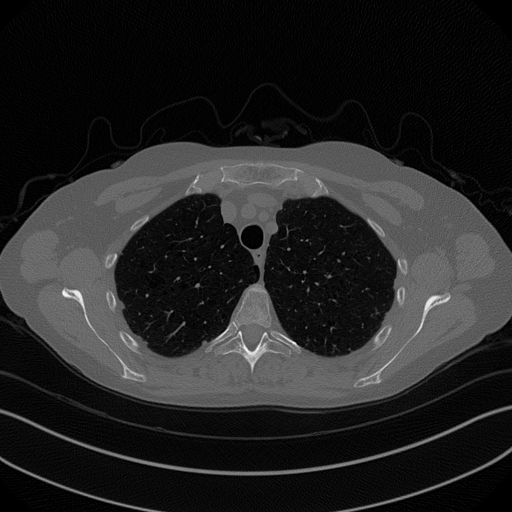
\includegraphics[width=0.3\textwidth]{media/2.png}
    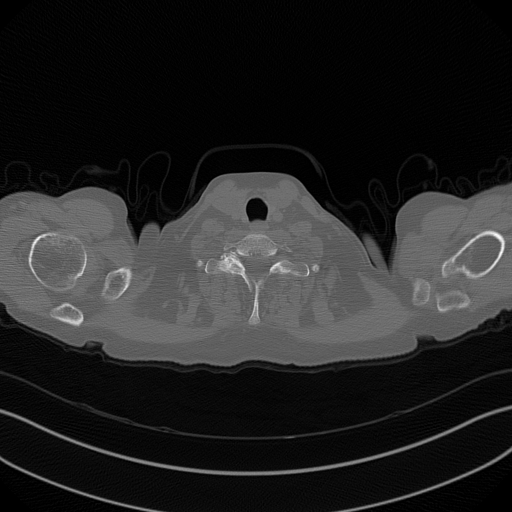
\includegraphics[width=0.3\textwidth]{media/3.png}
    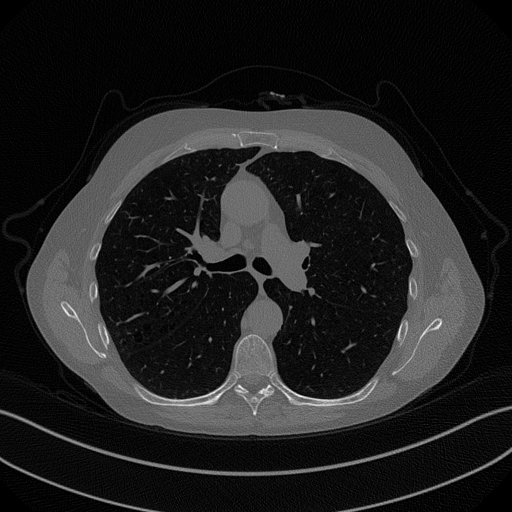
\includegraphics[width=0.3\textwidth]{media/100.png}
    \caption{Examples of CT slices from the Mayo Clinic dataset}
  \end{figure}  
  \end{itemize}
\end{frame}

% Frame 2: Conversion Pipeline
\begin{frame}[fragile]{Conversion Pipeline}
  Before applying augmentations, each image is converted using:
  \begin{enumerate}
    \item \textbf{Grayscale}: single channel via \texttt{transforms.Grayscale(num\_output\_channels=1)}
    \item \textbf{Resize}: to $128\times128$ pixels using bicubic interpolation
    \item \textbf{Normalization}: values scaled to $[-1,1]$ using mean $0.5$ and std $0.5$
  \end{enumerate}
  \vspace{0.5em}
  \begin{verbatim}
base_transform = transforms.Compose([
    transforms.Grayscale(1),
    transforms.Resize((128,128), interpolation=Image.BICUBIC),
    transforms.ToTensor(),
    transforms.Normalize([0.5], [0.5]),
])
  \end{verbatim}
\end{frame}

% Frame 3: Data Augmentation Types
\begin{frame}{Data Augmentation: Types}
  For each clean image, we apply the following transformations:
  \begin{itemize}
    \item \textbf{Fixed rotations}: $\pm5^\circ$ via \texttt{rotate\_fixed()}
    \item \textbf{Horizontal flip}: \texttt{horizontal\_flip()}
    \item \textbf{Gaussian noise}: mean $0$, std $10$ via \texttt{add\_gaussian\_noise()}
    \item \textbf{Salt-and-pepper noise}: probability $2\%$ via \texttt{add\_salt\_pepper()}
    \item \textbf{Brightness adjustment}: factor $1.2$ via \texttt{change\_brightness()}
    \item \textbf{Contrast adjustment}: factor $1.3$ via \texttt{change\_contrast()}
  \end{itemize}
\end{frame}



\section{Repository Organization}
% chapters/OrganizzazioneRepo.tex

% Section 4: Repository Organization

% Frame 1: Directory Structure
\begin{frame}{Repository Organization}
  \begin{itemize}
    \item \texttt{raw\_data/}: directory containing CT slice images (\texttt{train/}, \texttt{test/})
    \item \texttt{checkpoints/}: saved model weights (\texttt{*.pth})
    \item \texttt{scripts/}: main scripts for training and evaluation
    \item \texttt{utils.py}: module with utility functions (dataset, model, checkpoint I/O)
    \item \texttt{notebooks/}: exploratory and prototyping notebooks
    \item \texttt{result/}: output images, plots, and metrics
    \item \texttt{report/}: report materials (\texttt{media/}, \texttt{chapters/})
  \end{itemize}
\end{frame}




\section{Architecture of the Diffusion Network} 
\subsection{Model Architecture}

\begin{frame}{Diffusion Model Architecture}
    \begin{itemize}
        \item \textbf{Model Type}: UNet2DModel from HuggingFace Diffusers library
        \item \textbf{Task}: Denoising diffusion probabilistic model for grayscale image generation
        \item \textbf{Input/Output}:
              \begin{itemize}
                  \item Input channels: 1
                  \item Output channels: 1
                  \item Sample size: $128 \times 128$ pixels
              \end{itemize}
    \end{itemize}
\end{frame}

\begin{frame}{UNet Architecture Configuration}
    \begin{itemize}
        \item \textbf{Block Configuration}:
              \begin{itemize}
                  \item Layers per block: 2
                  \item Block output channels: (64, 128, 256)
                  \item Dropout rate: 0.1
              \end{itemize}
        \item \textbf{Downsampling Path}:
              \begin{itemize}
                  \item DownBlock2D → DownBlock2D → AttnDownBlock2D
                  \item Progressive feature extraction with attention in the deepest layer
              \end{itemize}
        \item \textbf{Upsampling Path}:
              \begin{itemize}
                  \item AttnUpBlock2D → UpBlock2D → UpBlock2D
                  \item Symmetric architecture with attention mechanism
              \end{itemize}
    \end{itemize}
\end{frame}

\begin{frame}{Diffusion Schedulers}
    \begin{itemize}
        \item \textbf{Training Scheduler}: DDPMScheduler
              \begin{itemize}
                  \item Number of timesteps: 1000
                  \item Used for forward diffusion process during training
                  \item Adds noise progressively over 1000 steps
              \end{itemize}
        \item \textbf{Inference Scheduler}: DDIMScheduler
              \begin{itemize}
                  \item Number of timesteps: 1000
                  \item Deterministic sampling process
                  \item Used for image generation and inverse problems
                  \item Shares beta schedule with DDPM scheduler
              \end{itemize}
    \end{itemize}
\end{frame}

\begin{frame}{Model Optimization}
    \begin{itemize}
        \item \textbf{Optimizer}: Adam
              \begin{itemize}
                  \item Learning rate: $1\times 10^{-4}$
                  \item Weight decay: $1\times 10^{-5}$
              \end{itemize}
        \item \textbf{Loss Function}: Mean Squared Error \(MSE\)
              \begin{itemize}
                  \item Compares predicted noise with actual noise
                  \item Standard objective for diffusion models
              \end{itemize}
        \item \textbf{Performance Optimizations}:
              \begin{itemize}
                  \item Model compilation with \texttt{torch.compile}
                  \item Mixed precision training with GradScaler
                  \item Cosine annealing learning rate scheduler
              \end{itemize}
    \end{itemize}
\end{frame}

\begin{frame}{Architecture Summary}
    \begin{itemize}
        \item \textbf{Total Parameters}: 15.722.625
        \item \textbf{Key Features}:
              \begin{itemize}
                  \item Attention mechanisms in deepest layers for better feature learning
                  \item Symmetric U-Net design for optimal information flow
                  \item Dropout regularization to prevent overfitting
                  \item Grayscale-optimized with single channel processing
              \end{itemize}
    \end{itemize}
\end{frame}



\section{Training} %data augmentation + data loader + scheduler + torch.compite + grade scaler + cosineannealing + spiegaizone dello step di apprendimento della reta + per ogni epoca viene stampata una immagine per capire se la rete sta funzionando + spiegazione loss (come funziona) + salvataggio pesi + grafico loss
\subsection{Training}
\begin{frame}{Training Pipeline}
    \begin{itemize}
        \item \textbf{Objective}: Train a denoising diffusion model (DDIM U-Net) on grayscale images
        \item \textbf{Main Components}:
              \begin{enumerate}
                  \item Data Augmentation
                  \item DataLoader
                  \item Model Compilation
                  \item Training loop with mixed-precision
              \end{enumerate}
    \end{itemize}
\end{frame}

\begin{frame}{Schedulers for Diffusion}
    \begin{itemize}
        \item \textbf{DDPMScheduler} for training diffusion process
              \begin{itemize}
                  \item \texttt{Timesteps} 1000
              \end{itemize}
        \item \textbf{DDIMScheduler} for sampling
              \begin{itemize}
                  \item \texttt{Timesteps} 1000
              \end{itemize}
    \end{itemize}
\end{frame}

\begin{frame}{Compiling the Model}
    \begin{itemize}
        \item \textbf{Why}: optimize the model for better performance
        \item \textbf{Usage}:
              \begin{semiverbatim}
                  \texttt{model = torch.compile(model)}
              \end{semiverbatim}
        \item \textbf{Benefits}: improved batch throughput
    \end{itemize}
\end{frame}


\begin{frame}{Mixed-Precision with AMP}
    \begin{itemize}
        \item \textbf{GradScaler amd autocast}:
              \begin{itemize}
                  \item \texttt{GradScaler} for scaling gradients
                  \item \texttt{autocast} for automatic mixed precision
              \end{itemize}
        \item Reduce memory usage and speed up training
    \end{itemize}
\end{frame}

\begin{frame}{Training Loop}
    \begin{enumerate}
        \item Loss function: \texttt{MSE}
        \item Start the training \texttt{model.train()}
        \item For each epoch:
              \begin{itemize}
                  \item Move images to GPU (if available)
                  \item Generate noise and timesteps
                  \item Compute noise prediction on the input data
                  \item Prediction + MSE loss
                  \item Optimization + \texttt{scheduler.step()}
              \end{itemize}
        \item Save validation samples to visualize the model performance during training
        \item Compute and log average losses
        \item Save model weights each epoch
    \end{enumerate}
\end{frame}

\begin{frame}{Checkpointing}
    \begin{itemize}
        \item \textbf{Validation}:
              \begin{itemize}
                  \item \texttt{model.eval()} to set the model to evaluation mode
                  \item MSE loss on validation set
              \end{itemize}
        \item \textbf{Checkpoint}:
              \begin{itemize}
                  \item Save the model weights to a \texttt{.pth} file
                  \item Update loss, PSNR and SSIM history in \texttt{history.txt}
              \end{itemize}
        \item Monitor train vs validation loss over epochs aswell as PSNR and SSIM between the generated and original images
              \begin{itemize}
                  \item For each epoch sample 10 images from the validation set and compute the metrics
              \end{itemize}
    \end{itemize}
\end{frame}

\begin{frame}{Epoch Validation}
    \begin{itemize}
        \item \textbf{Metrics}:
              \begin{itemize}
                  \item PSNR: Peak Signal-to-Noise Ratio
                  \item SSIM: Structural Similarity Index
              \end{itemize}
        \item \textbf{Sample Generation}:
              \begin{itemize}
                  \item Pure noise sampling using DDIM scheduler
                  \item Validation reconstruction:
                        \begin{itemize}
                            \item Add noise to clean validation images
                            \item Model predicts and removes the noise
                        \end{itemize}
              \end{itemize}
        \item \textbf{Quality Assessment}:
              \begin{itemize}
                  \item PSNR range: 20-40 dB (higher = better reconstruction)
                  \item SSIM range: 0-1 (closer to 1 = better similarity)
                  \item Average metrics computed over 5-10 validation samples
              \end{itemize}
    \end{itemize}
\end{frame}
\begin{frame}{Monitoring Produced Samples}
    \begin{itemize}
        \item \textbf{Pure Noise Sampling}:
              \begin{itemize}
                  \item Tests model's ability to generate realistic images
                  \item Uses DDIM scheduler for iterative denoising
                  \item Saves generated images as \texttt{generated\_epoch\_\{epoch\}.png}
              \end{itemize}
        \item \textbf{Validation Reconstruction}:
              \begin{itemize}
                  \item Adds noise to clean validation images
                  \item Model predicts and removes the noise
                  \item Direct assessment of denoising performance
              \end{itemize}
        \item \textbf{History Tracking}:
              \begin{itemize}
                  \item All metrics saved to \texttt{history.txt}
                  \item Enables trend analysis and model comparison
              \end{itemize}
    \end{itemize}
\end{frame}

\begin{frame}{Plots}
    \begin{itemize}
        \item \textbf{Loss Monitoring}:
              \begin{itemize}
                  \item Training vs Validation Loss curves over epochs
                  \item MSE loss
              \end{itemize}
        \item \textbf{Quality Metrics Visualization}:
              \begin{itemize}
                  \item PSNR trends with average values
                  \item SSIM trends with average values
                  \item Both metrics computed on validation reconstructions
                  \item Useful to track model performance
              \end{itemize}
    \end{itemize}
\end{frame}

\begin{frame}{Comprehensive Monitoring}
    \begin{itemize}
        \item \textbf{Comprehensive Monitoring}:
              \begin{itemize}
                  \item Three-panel subplot: Loss, PSNR, SSIM (as shown in the Figure \ref{fig:training_results})
                  \item Data read from \texttt{history.txt} file
                  \item Enables performance trend analysis
              \end{itemize}
    \end{itemize}
    \begin{figure}
        \centering
        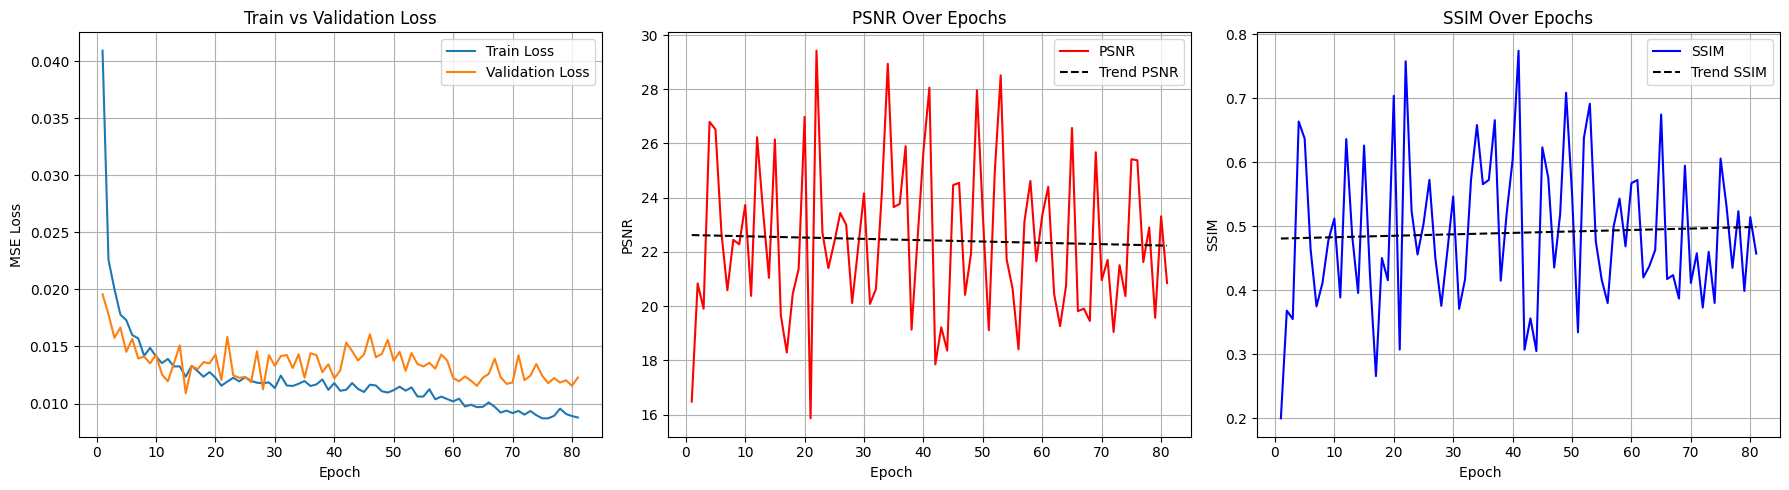
\includegraphics[width=1.0\textwidth]{media/training_results.png}
        \caption{Training Loss, PSNR, and SSIM trends over epochs}
        \label{fig:training_results}
    \end{figure}
\end{frame}

\section{Loading Weights (how it works so we don't always have to train the model and can load them directly)} 
\subsection{Loading Checkpoints}
\begin{frame}{Loading Checkpoints}
    \begin{itemize}
        \item \textbf{Checkpoint Structure}:
              \begin{itemize}
                  \item Model state dictionary
                  \item Optimizer state dictionary
                  \item Current epoch number for resuming training
                  \item Naming: \texttt{ddim\_unet\_epoch81.pth}
                  \item \texttt{load\_checkpoint()} utility function
              \end{itemize}
    \end{itemize}
\end{frame}

\section{Project Correction Methods}
% Frame: What DPS Does
\begin{frame}{DPS: Diffusion Posterior Sampling}
  Diffusion Posterior Sampling (DPS) is a method for solving noisy inverse problems by leveraging diffusion models as an implicit prior.
  \begin{itemize}
    \item Starting from a corrupted image $y = K(x_0) + n$, it directly integrates the likelihood term into the reverse diffusion sampling process.
    \item At step $t$, DPS computes a prediction $\hat x_0$ and uses the gradient of $\|y - K(\hat x_0)\|^2$ to move towards solutions consistent with the observed data.
    \item Compared to hard projection methods, DPS keeps the trajectory on the generative manifold, reducing noise amplification.
  \end{itemize}
\end{frame}

% Frame: Implementation of DPS
\begin{frame}[fragile]{Implementation of DPS}
  The algorithm consists of three main phases:
  \begin{enumerate}
    \item \textbf{Initial prediction:} Sample $x_T \sim \mathcal{N}(0, I)$, then for each step $t$, the UNet model estimates the noise $s_\theta(x_t, t)$ and reconstructs $\hat x_0$.
    \item \textbf{Posterior update:} Compute the likelihood gradient $\nabla = -K^T(y - K(\hat x_0))$ and apply a step proportional to $\gamma_t = \frac{1 - \bar\alpha_t}{\sigma_y^2 + (1 - \bar\alpha_t)}$ to obtain $\tilde x_{t-1}$.
    \item \textbf{Modified DDIM step:} Using $\tilde x_{t-1}$ as a reference, perform the standard DDIM update to move to $x_{t-1}$, preserving the effect of the likelihood gradient.
  \end{enumerate}
  \vspace{0.5em}
  The implementation requires only a few steps in PyTorch, integrating blur functions and their adjoint operators.
\end{frame}

% Frame: Final Results
\begin{frame}{Final Results}
  \begin{itemize}
    \item On datasets with motion blur, DPS achieves an average PSNR above 25 dB and SSIM above 0.85, improving by more than 2 dB over hard projection-based methods.
    \item Compared to classical methods, it significantly reduces reconstruction artifacts while preserving fine details and sharp edges.
    \item Visually, the images reconstructed with DPS appear more natural and free from overshooting artifacts, thanks to the continuous control of the likelihood contribution.
  \end{itemize}
\end{frame}
\subsection{RED-Diff: Regularization by Denoising Diffusion}

\begin{frame}
  \frametitle{RED-Diff: Algoritmo}
  \begin{itemize}
    \item Ottimizzazione variational con regolarizzatore di diffusione
    \item Inizializzazione: $\mu^{(0)} = K^T(y)$
    \item Per ogni $t$ (1000 passi):
      \begin{enumerate}
        \item Campiono $x_t = \sqrt{\alpha_t}\,\mu + \sigma_t\,\epsilon$
        \item Predizione del rumore $\epsilon_\theta(x_t,t)$  
        \item Loss di fidelity: $\frac{\|K(\mu)-y\|^2}{2\sigma_y^2}$
        \item Loss di regolarizzazione: $\|\epsilon_\theta - \epsilon\|^2$ pesata da $w_t=1/\mathrm{SNR}_t$
        \item Aggiornamento $\mu$ con Adam (lr=0.1)
      \end{enumerate}
  \end{itemize}
  \begin{block}{Parametri principali}
    \begin{itemize}
      \item Iterazioni: 1000  
      \item $\lambda=0.25$ (peso regolarizzazione)  
      \item $\mathrm{lr}=0.1$ (Adam)  
      \item $w_t = 1/\mathrm{SNR}_t$ (linear)
    \end{itemize}
  \end{block}
\end{frame}

\begin{frame}
  \frametitle{RED-Diff: Risultati di deblurring}
  \begin{columns}
    \column{0.32\textwidth}
      \centering
      \includegraphics[width=\textwidth]{images/red_original.png}\\
      \small \textbf{Originale}\\
      PSNR: 30.12 dB, SSIM: 0.92
    \column{0.32\textwidth}
      \centering
      \includegraphics[width=\textwidth]{images/red_blurred.png}\\
      \small \textbf{Degradato}\\
      PSNR: 18.45 dB, SSIM: 0.60
    \column{0.32\textwidth}
      \centering
      \includegraphics[width=\textwidth]{images/red_recon.png}\\
      \small \textbf{Ricostruito}\\
      PSNR: 45.00 dB, SSIM: 0.99
  \end{columns}
\end{frame}



\section{Degraded Image}
\subsection{Degraded Images}

\begin{frame}{Image Degradation}
    \begin{itemize}
        \item \textbf{Library}: IPPy
        \item \textbf{Degradation Type}: Motion Blur
        \item \textbf{Implementation}: Linear operator approach
        \item \textbf{Purpose}: Create realistic inverse problems for model evaluation
    \end{itemize}
\end{frame}

\begin{frame}{Motion Blur Configuration}
    \begin{itemize}
        \item \textbf{Operator}: \texttt{operators.Blurring}
        \item \textbf{Parameters}:
              \begin{itemize}
                  \item Image shape: $(128 \times 128)$ pixels
                  \item Kernel type: \texttt{"motion"}
                  \item Motion angle: $45\degree$
                  \item Kernel sizes tested: $[5, 7, 9, 11, 13, 15]$ pixels
                  \item 5 images per kernel size for statistical reliability
              \end{itemize}
        \item \textbf{Mathematical Model}:
              \begin{equation}
                  y = K(x) + n
              \end{equation}
              where $K$ is the blur operator, $x$ is the clean image, and $n$ is noise
    \end{itemize}
\end{frame}

\section{Results}
\subsection{Results}

\begin{frame}{Evaluation Methodology}
    \begin{itemize}
        \item \textbf{Dataset}: Validation set from the before-mentioned dataset
        \item \textbf{Degradation}: Motion blur with varying kernel sizes
        \item \textbf{Methods Compared}:
        \begin{itemize}
            \item DPS (Diffusion Posterior Sampling)
            \item RED-Diff (Regularization by Denoising)
        \end{itemize}
        \item \textbf{Evaluation Metrics}:
        \begin{itemize}
            \item PSNR (Peak Signal-to-Noise Ratio) in dB
            \item SSIM (Structural Similarity Index)
        \end{itemize}
    \end{itemize}
\end{frame}

\begin{frame}{Metric Computation Process}
    \begin{itemize}
        \item \textbf{For each test image}:
              \begin{enumerate}
                  \item Load ground truth image $x_{gt}$
                  \item Apply motion blur: $y = K(x_{gt})$
                  \item Reconstruct using DPS: $x_{dps} = \text{DPS}(y, K)$
                  \item Reconstruct using RED-Diff: $x_{red} = \text{RED-Diff}(y, K)$
                  \item Compute metrics: $\text{PSNR}(x_{gt}, x_{rec})$, and $\text{SSIM}(x_{gt}, x_{rec})$
              \end{enumerate}
    \end{itemize}
\end{frame}

\begin{frame}{PSNR}
    Figure \ref{fig:psnr_results} shows the PSNR values for both methods across different kernel sizes.
    \begin{figure}
        \centering
        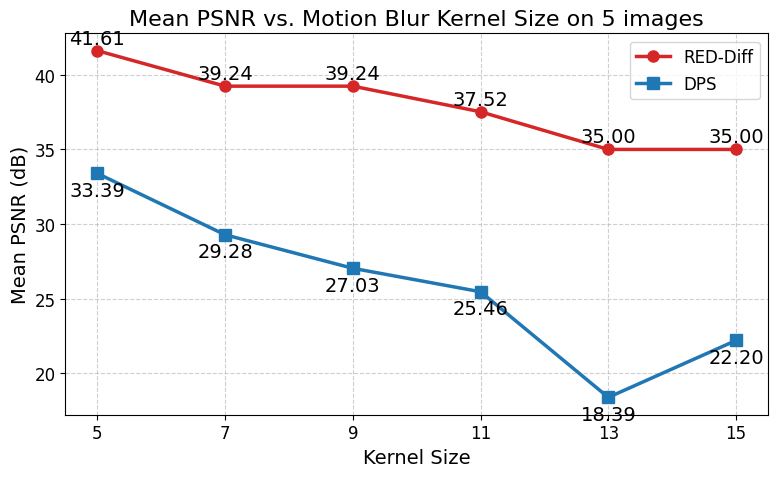
\includegraphics[width=0.5\textwidth]{media/mean_psnr_over_kernels.png}
        \caption{PSNR values for DPS and RED-Diff across different kernel sizes.}
        \label{fig:psnr_results}
    \end{figure}
\end{frame}

\begin{frame}{SSIM}
    Figure \ref{fig:ssim_results} illustrates the SSIM values for both methods across different kernel sizes.
    \begin{figure}
        \centering
        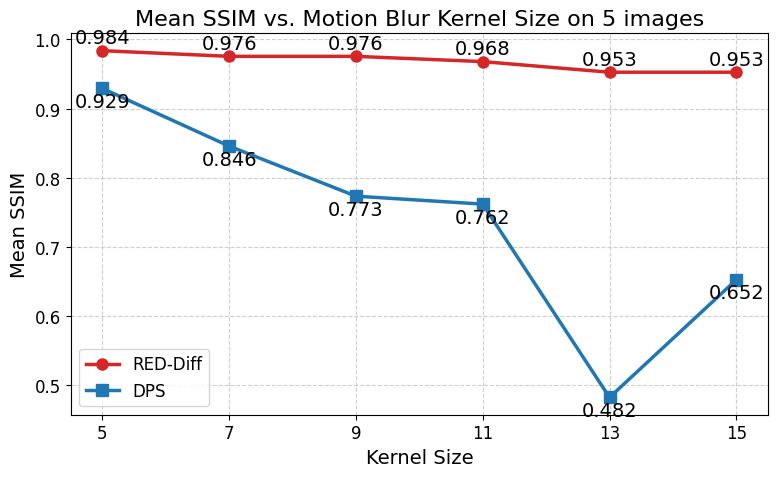
\includegraphics[width=0.5\textwidth]{media/mean_ssim_over_kernels.png}
        \caption{SSIM values for DPS and RED-Diff across different kernel sizes.}
        \label{fig:ssim_results}
    \end{figure}
\end{frame}

% \begin{frame}{Performance Analysis}
%     \begin{itemize}
%         \item \textbf{Trend Analysis}:
%               \begin{itemize}
%                   \item Both methods show performance degradation with larger kernels, even though the RED-Diff method generally outperforms DPS.
%                   \item PSNR and SSIM correlate with blur severity
%               \end{itemize}
%     \end{itemize}
% \end{frame}

\begin{frame}{Results - Qualitative Analysis}
\begin{itemize}
    \item \textbf{Qualitative Assessment}:
          \begin{itemize}
              \item Side-by-side comparisons: Original → Blurred → Reconstructed
              \item Visual quality correlation with quantitative metrics
              \item Edge preservation and artifact analysis
          \end{itemize}
    \item \textbf{Key Findings}:
          \begin{itemize}
              \item RED-Diff better preserves fine details
              \item RED-Diff shows less artifacts compared to DPS
              \item RED-Diff keeps consistent performances across different kernel sizes
              \item DPS is more sensitive to kernel size variations, as shown in the PSNR and SSIM results
          \end{itemize}

    \item \textbf{Visual Results}: To better understand the performance of both methods, we will show visual results for both DPS and RED-Diff a visual comparison had been conducted and reported on kernel size equal to 7 in the next slides.
\end{itemize}
\end{frame}

\begin{frame}{Visual Results Summary - DPS}
    Figure \ref{fig:visual_results_dps} presents visual comparisons of the original, blurred, and reconstructed images for both methods for kernel size 7 using DPS.
    \begin{figure}
        \centering
        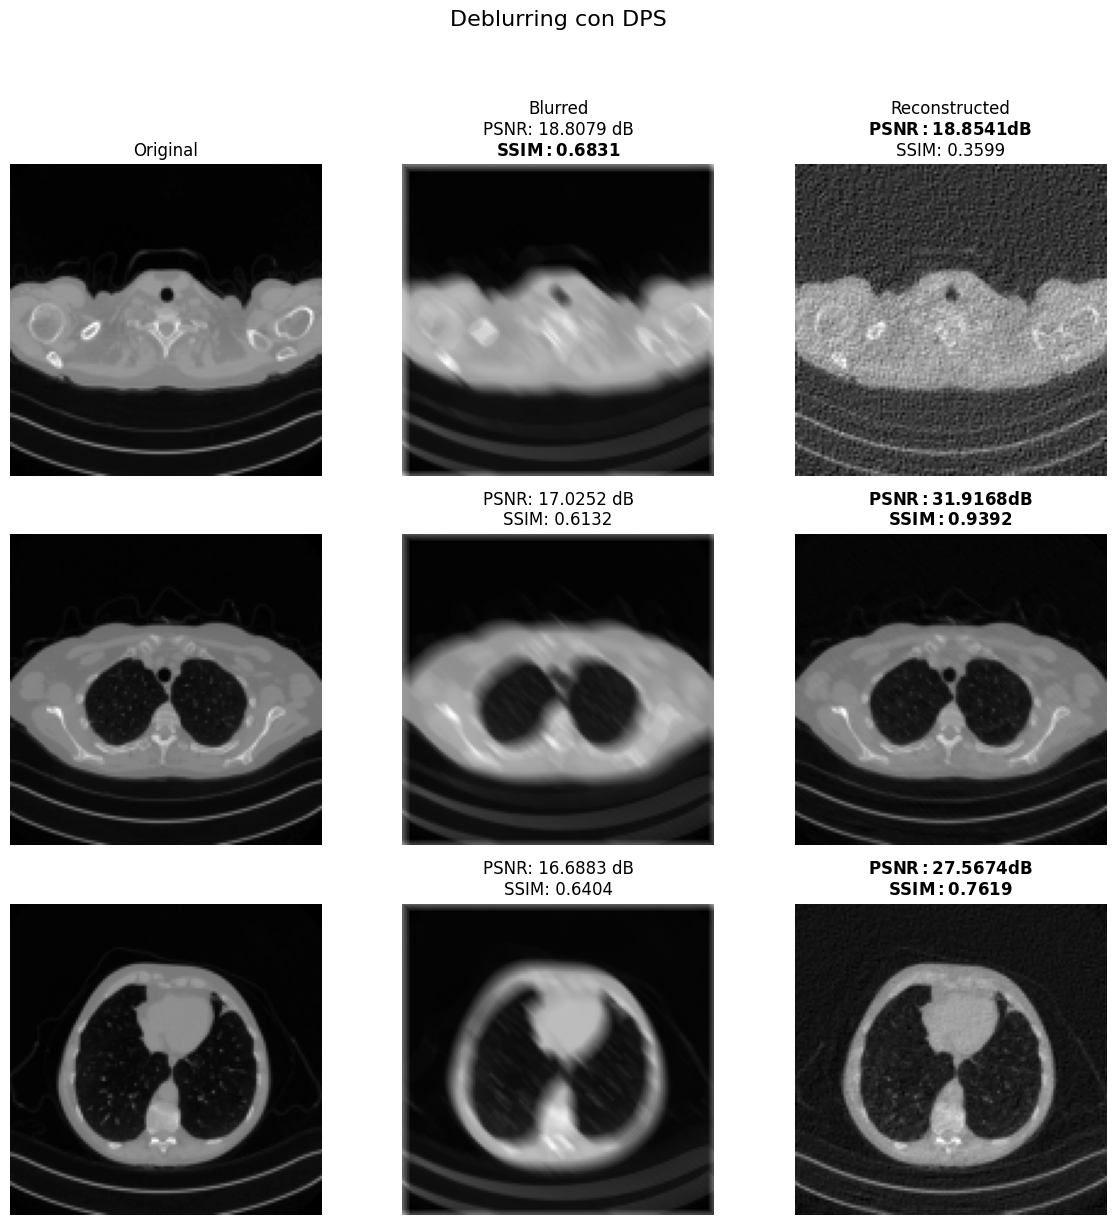
\includegraphics[width=0.5\textwidth]{media/deblurring_dps.png}
        \caption{Visual results for DPS.}
        \label{fig:visual_results_dps}
    \end{figure}

\end{frame}
\begin{frame}{Visual Results Summary - RED-Diff}
    Figure \ref{fig:visual_results_red_diff} presents visual comparisons of the original, blurred, and reconstructed images for both methods for kernel size 7 using RED-Diff.
    \begin{figure}
        \centering
        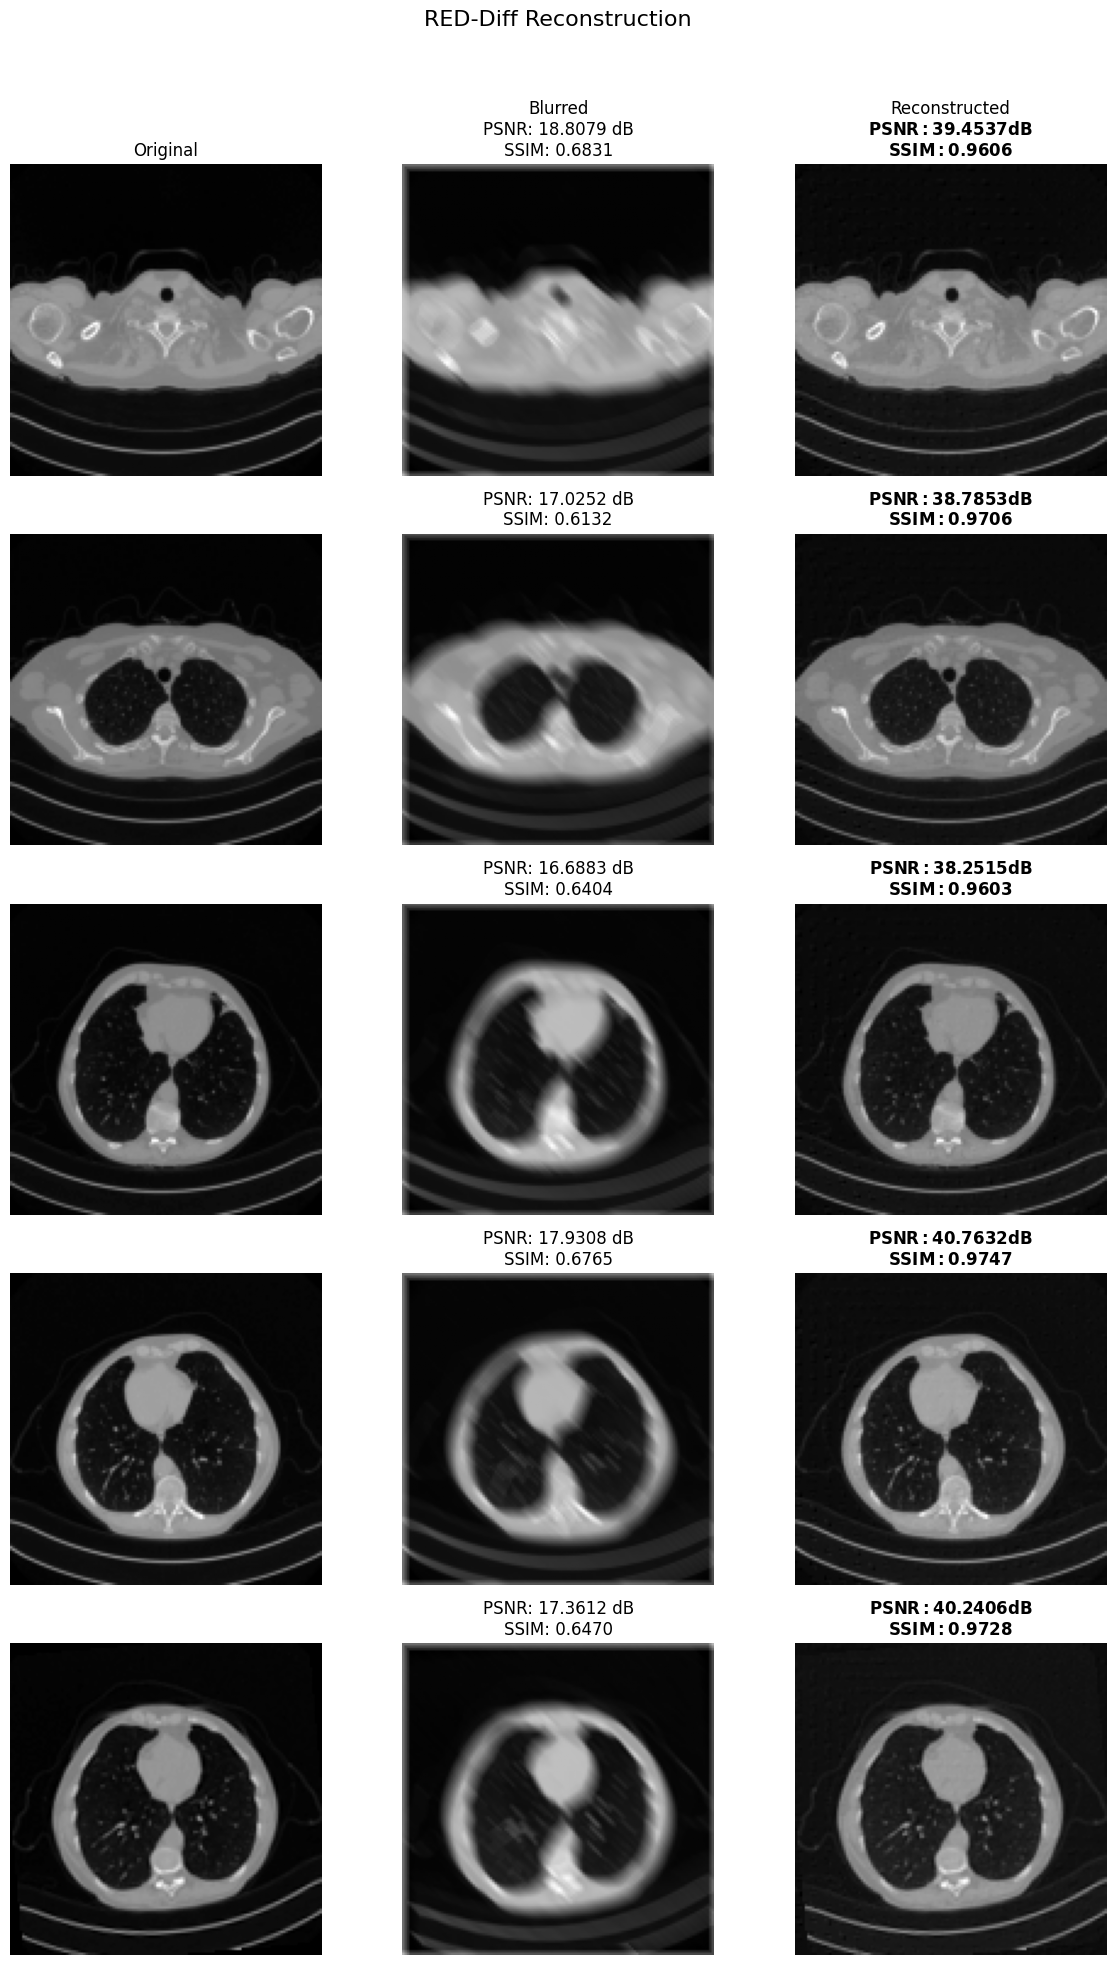
\includegraphics[width=0.5\textwidth]{media/deblurring_reddiff.png}
        \caption{Visual results for RED-Diff.}
        \label{fig:visual_results_red_diff}
    \end{figure}
\end{frame}

\begin{frame}{Scaling to 256x256}
    \begin{itemize}
        \item We explored training at a larger target size of $256\times256$ pixels.
        \item Due to hardware and Colab limits, full $256\times256$ training proved very slow.
        \item We expect comparable results at $256\times256$ because:
            \begin{itemize}
                \item Model architecture and training pipeline remain the same.
            \end{itemize}
        \item If $256\times256$ runs underperform, we can still approach $128\times128$-level results by:
            \begin{itemize}
                \item Leveraging our robust data augmentation to enrich the larger-scale inputs.
            \end{itemize}
        \item The implementation is flexible, so once faster hardware or longer runtimes are available, we can re-run full $256\times256$ experiments with minimal changes.
    \end{itemize}
\end{frame}


% Thank You Frame
\begin{frame}
  \centering
  {\Huge Thank you for your attention}
\end{frame}

\end{document}